\chapter{Propiedades colectivas}

\section{Fomra nuclear y multipolaridad}

\subsection{Momento cuadrupolar eléctrico}

\subsection{Momento dipolar magnético}

\section{Geometría de núcleos par-par}

\subsection{Modos de vibración}

Podemos definir diferentes modos de vibración alrededor de la esfera:

\begin{figure}[h!] \centering
    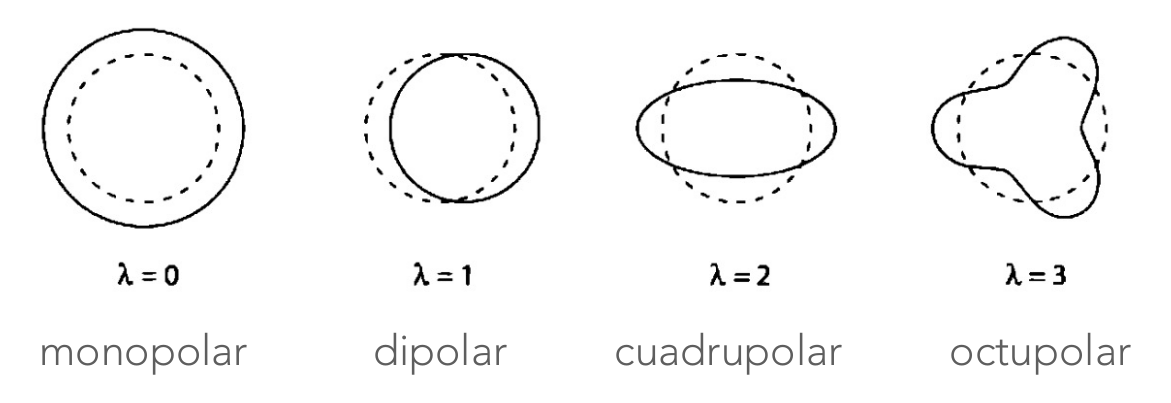
\includegraphics[width=0.9\linewidth]{Cuerpo/Ch_02/02_Modos_Vibracion.png}
\end{figure}
El cuanto de energía vibracional es el fonón. Si añadimos un fonón de modo $\lambda=2$ (fonón cuadrupolar) a un estado fundamental $0^+$, el resultado es un estado $2^+$, ya que añade una componente $Y_{2\mu}$ a la función de ondas. 


\subsection{Rotación nuclear}

La superficie de cualquier sólido puede describirse a través de los armónicos esféricos. Si nos centramos en formas cuadrupolares no triaxiales, 

\section{Deformación nuclear en el modelo de capas}

\subsection{Modelo de Nilsson}

\subsection{Correción de capas de Strutinsky}


\section{Apareamiento de nucleones}

\subsection{Seniority}


\subsection{Aproximación BCS}

